\documentclass{article}
\usepackage{graphicx} % Required for inserting images
\usepackage{svg} % Required for inserting images
\usepackage[pdfborder={0 0 0}]{hyperref}    % turns references into hyperlinks
\usepackage[margin=25mm]{geometry}  % adjusts page layout
\usepackage{amsmath}
\usepackage{xspace}  %
\usepackage{caption}
\usepackage{subcaption}
\usepackage{minted}
\usepackage{algorithm}
\usepackage{enumitem}
\usepackage{tabularray}
\usepackage{tablefootnote}
\usepackage{makecell}
\usepackage[T1]{fontenc}
\parskip=3pt

\renewcommand\theadalign{bc}
\renewcommand\theadfont{\bfseries}

\DeclareMathOperator{\sinc}{sinc}
\newcommand{\sectionref}[1]{\hyperref[sec:#1]{Section~\ref*{sec:#1}}}

\captionsetup[figure]{justification=centering}

\title{Reconstruction of displayed text from electromagnetic emissions of a digital video cable}
\author{Balázs Tóth}
\date{6 December 2023}

\begin{document}

\maketitle

\begin{center}
    Word count: 
\end{center}


\section{Introduction}
When transferring data via a High-Definition Multimedia Interface (HDMI) cable, it emits electromagnetic radiation. This electromagnetic radiation can then be captured by a receiving antenna in the vicinity of the cable, and digital signal processing methods can be applied to the sampled data to reconstruct the original information transmitted via the HDMI cable.

We have been provided with $1$ second long IQ downconverted recordings of the 205-495 MHz radio spectrum near a computer with HDMI display courtesy of Dr Markus Kuhn. The HDMI cable is transmitting the $640 \times 480$ image shown in \autoref{fig:original} at $60$ frames a second.

\begin{figure}[htb]
\centering
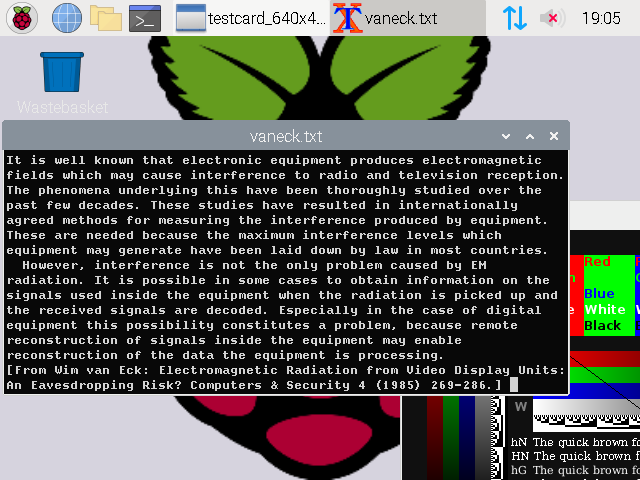
\includegraphics[width=0.7\linewidth]{figures/scene3-640x480.png}
\caption{The original image we wish to reconstruct.}
\label{fig:original}
\end{figure}

This report gives the details of an implementation which transforms these IQ downconverted recordings, back into a human-readable image.


\section{Implementation}
\label{sec:implementation}

The entire project was implemented in \texttt{Pluto} notebooks using \texttt{Julia} and its \texttt{DSP}, \texttt{Plots}, \texttt{FFTW}, \texttt{ImageIO}, \texttt{ImageShow}, and \texttt{Statistics} libraries. All of the code written is available at \url{https://github.com/bazsi700/dsp-assignment4a}.

The following sections detail the implementation steps completed in order to achieve the image reconstructions in \sectionref{results}. We use the following list of terminology in the sections to come:
\begin{itemize}[noitemsep,topsep=0pt]
    \item $f_c$ is the centre frequency of the sampling
    \item $f_s$ is the sampling frequency
    \item $t_s = f_s^{-1}$ is the sampling period
    \item $x_t \times y_t$ is the number of pixels transmitted per frame
    \item $f_p$ is the pixel clock frequency
    \item $f_h$ is the number of lines transmitted per second
    \item $f_v$ is the number of frames transmitted per second
    \item $\{z_n\}$ are the samples of the IQ downcoverted recording.
\end{itemize}

\subsection{Resampling and displaying image}
\label{sec:resampling}

As the recorded data is sampled with a sampling frequency of $f_s = 64$Mhz, but pixels are transmitted at a frequency of $f_p \simeq 25.175$MHz, we want to resample the data, so that each element corresponds to one pixel. To do this resampling, we try three different algorithms:

\begin{description}

\item[Nearest neighbour sampling] Here for each resampled point, we simply pick the original data point closest to it in time and use the value of that.
\item[Linear] For each resampled point, we pick the two closest original samples and weigh them linearly by their distance.
\item[Windowed sinc] This is an approximation to the sinc reconstruction, which would yield a perfect reconstruction (as the data satisfies the Nyquist limit). To approximate the exact reconstruction, we use a window size of $2k+1$, and we set the resampled value to 
$$
\sum\limits_{j=-k}^{k}z_{i+j} \cdot \sinc(t - (i+j) t_s)
$$
where $t$ is the resampled time, and $i$ is the index in the original data closest to $t$.
 
\end{description}

We found that linear resampling gave the best results, and hence use that for the rest of this report.

After resampling, we can simply display a greyscale image, by splitting it into rows of $y_t$ samples, taking the absolute value of every element, and using it as the intensity level in a greyscale image. To make the image actually visible, we normalize all intensity values, by rescaling the maximum intensity to 1.

To get a better image quality, we also use a higher resampling rate of $f_r = m \cdot f_p$. This way, for each pixel we have $m$ samples and get a higher resolution image. In order for the displayed image not to be distorted, we use a height:width ratio of $m:1$, and essentially display every row $m$ times. Empirically, $m=3$ provided a good trade-off between running time and image quality so we use that for the rest of the report.

\subsection{Removing shearing}
\label{sec:shearing}

Using a resampling rate of $f_p = 25.175$MHz, we get visible shearing of the picture, as the resampling rate does not exactly match the actual pixel transmission rate, shown in \autoref{fig:251750fs}. By experimentation, we notice that a resampling rate of $25.2$MHz gives decent image quality within one frame, however, across multiple images we still get shearing as seen in \autoref{fig:252000fs}.

\begin{figure}[htb]
\centering
\raisebox{40pt}{
\begin{subfigure}[t]{.475\textwidth}
    \centering
    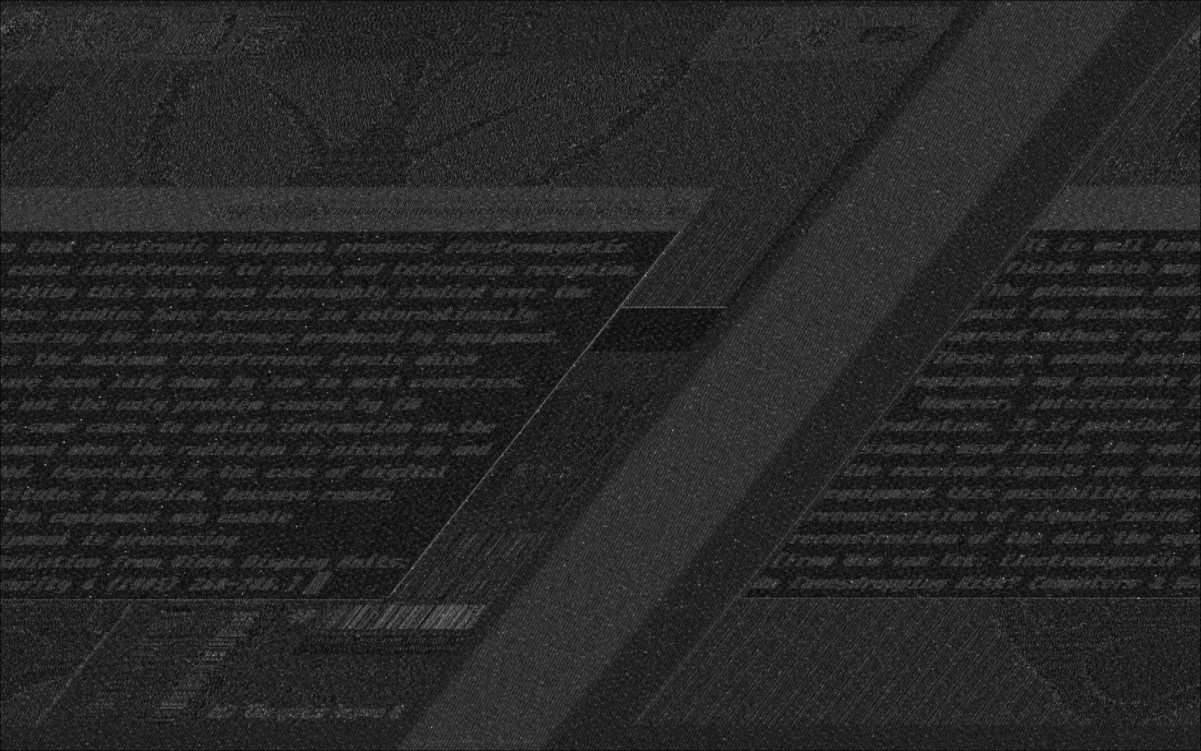
\includegraphics[width=\linewidth]{figures/251750fs.png}
    \caption{One frame with $f_s = 25.175$MHz}
    \label{fig:251750fs}
\end{subfigure}
}
\hfill
\begin{subfigure}{.475\textwidth}
    \centering
    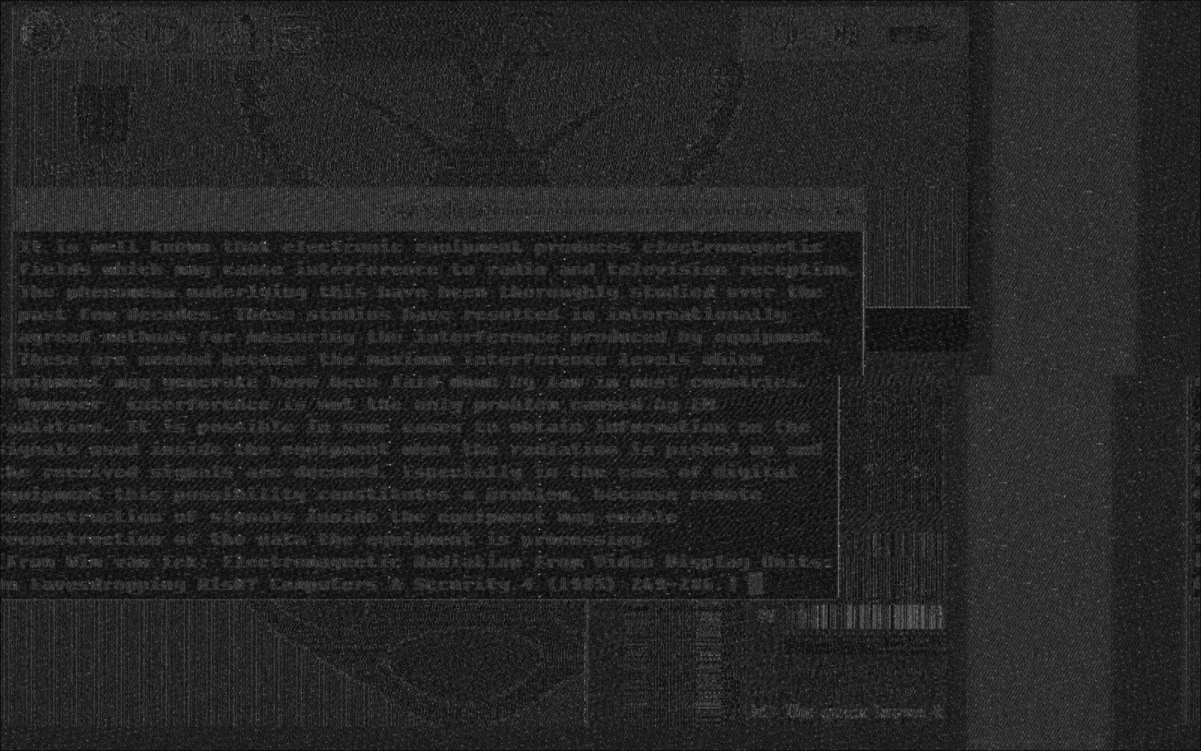
\includegraphics[width=\linewidth]{figures/252000fs.png}
    \caption{Shearing across multiple frames with $f_s = 25.2$MHz. The top half of the image is from the first frame, and the bottom half is from 10 frames later.}
    \label{fig:252000fs}
\end{subfigure}

\caption{Shearing we get with different naive $f_s$ values}
\label{fig:shearing}
\end{figure}

To resolve this, we resort to the auto-correlation sequence of the original data. This sequence will have huge peaks every $f_s \cdot f_v^{-1}$ elements, as these are the offsets corresponding to an integer number of frames, and the transmitted frame is the same every $f_v^{-1}$ seconds. 

To exploit this feature, we use the heuristic, that each of these peaks is going to be a local maximum in the auto-correlation sequence, satisfying that it is greater than every element between it and the neighbouring peaks. We use the following code to locate the peaks satisfying this property:

\begin{center}
\begin{minted}{julia}
abs_iq = abs.(iq)
corr = xcorr(abs_iq,abs_iq)
leng = length(corr)

# the midpoint is the crosscorrelation with offset 0
midpoint = round(Int,(length(corr)+1)/2)

# The offset 0 is the first frame
frame_inds = zeros(1)	

# For each offset we check in what neighbourhood it is maximal
# if it's at least 6e5 it is the offset of a frame

for i in 1:Int(25e6) # 45e5 for merged
    closest_bigger = 0
    for j in 1:midpoint
        if corr[midpoint+i-j] > corr[midpoint+i] || 
           corr[midpoint+i+j] > corr[midpoint+i]
            closest_bigger = j
            break
        end
    end
    if closest_bigger > 6e5 # 18e5 for merged
        append!(frame_inds,i)
    end
end

mean_diff = mean(frame_inds[2:end] .- frame_inds[1:end-1])
fv = fs/mean_diff
\end{minted}
\end{center}

Empirically we find, that using around 20 frames worth of samples, the above-described heuristic holds, and each peak will correspond to a different frame. Averaging out the distances between the peaks we get an estimate for $f_v$ accurate enough to maintain horizontal alignment between all of the frames using the resampling rate of $f_p = f_v \cdot x_t \cdot y_t$. We also use non-coherent auto-correlation as empirically it seems to give better results for low noise contents, however, we switch to coherent auto-correlation in noisier environments.

Removing shearing also allows us to non-coherently average out all frames in the recording to reduce the noise, as these will average out to a relatively smooth small value, while the actual data will be preserved properly in all the frames. Using coherent averaging with greyscale images results in significantly worse image quality, as the phases of the same pixel in different frames cancel out, removing the information content.

\subsection{Alignment}
\label{sec:alignment}

The recordings start at an arbitrary point in time, not at the beginning of a frame, thus the previously reconstructed image is going to be shifted both horizontally and vertically. We want to resolve this by dropping a number of samples from the beginning so that the first sample corresponds to the top-left corner of the image.

The original transmitted picture is $640 \times 480$ pixels at $60$Hz, however, the HDMI cable actually transmits $800 \times 525$ pixels for each frame, as horizontal and vertical blanking periods are added for synchronisation, and so that the display device can catch up to the data. 

Perusing the VESA DMT standard\footnote{\url{https://glenwing.github.io/docs/VESA-DMT-1.13.pdf}, page 21} we can see that these blanking periods consist of a syncing period, some borders to the frame and a front and back porch. We use the heuristic which seems to work quite well empirically, that these blanking periods will have a lower standard deviation than the image content of the frame.

For alignment in both directions, we first resample the data with the previously found $f_p$ value and construct the matrix of frames. Then we take the mean of overlapping blocks of $2$ frames over $16$ frames to get a sufficiently long sample with reduced noise content. Then for horizontal alignment, we take a rolling window of $160$ columns (the length of the horizontal blanking period) and take the standard deviation over these windows for all $800$ possible offsets. We can then locate the minimum of the standard deviations, and by finding the end of that window, we find the end of the blanking period, i.e. the start of a new line. |

For vertical alignment, we first cyclically rotate the image, so that the start of the rows coincides with the start of a line in the HDMI transmission. Then we only consider the first $525$ samples in each row, as excluding the horizontal blanking period better shows the difference between image lines and blanking lines. After this, similarly to the horizontal case, we take the standard deviations over a rolling window of $45$ rows (the length of the vertical blanking period) and find the offset with minimal standard deviation. \autoref{fig:stds} shows the graph of standard deviations for each window offset for both horizontal and vertical alignment.

After finding the correct horizontal offset of $o_h$, and vertical offset of $o_v$ of the image, we can drop the first $\left(o_v \cdot x_t + o_h\right) \cdot \frac{f_s}{f_p}$ samples from the original IQ recording for all future reconstructions.

\begin{figure}[htb]
\centering
\begin{subfigure}{.475\textwidth}
    \centering
    \includesvg[width=\linewidth]{figures/column_std.svg}
\end{subfigure}
\hfill
\begin{subfigure}{.475\textwidth}
    \centering
    \includesvg[width=\linewidth]{figures/row_std.svg}
\end{subfigure}

\caption{Rolling window standard deviations of columns and rows for different offsets. The minima correspond to the windows overlapping the blanking periods.}
\label{fig:stds}
\end{figure}

For unknown reasons, this above-described alignment finding fails for the centre frequency of $350$ and $375$MHz, despite the data not being overly noisy, as the standard deviations including the actual image as well are relatively small too. To solve this issue, instead of a window size of $160$, we use a window size of $48$ which is the total length of the horizontal back porch and left border in the VESA standard, which results in a sharp local minimum in the standard deviations. However, the longer, $96$ pixel long syncing period has a lower standard deviation in its window. To combat this, instead of finding the minimum, we find the index $i$ maximising $(s_{i+10}-s_i) \cdot (s_{i-10}-s_i)$ where $s_n$ is the standard deviation of the window with offset $n$. This exploits the fact that the local minimum corresponding to the back porch and left border is very sharp, and hence in both directions it is surrounded by values greater than it. This method allows us to get a correct alignment for $375$MHz as well. This alternative method does not work everywhere either, as for low frequencies with more noise the former simpler method gives better results, thus we are forced to switch between the two.

\subsection{Unrotating phase}

Instead of taking the absolute value of each complex pixel value and displaying it as a greyscale image, we can instead keep the phase information and display it as hue, while still using the absolute value as brightness in the HSV colour space. Alternatively, the real part could be used as the red channel and the imaginary part as the green channel, however, we found that the HSV representation results look visually nicer, and hence decided to use those for the rest of this report. We also increase the brightness values of the images by various manually set values before normalizing them to have a maximum of 1, in order to get better images.

Naively displaying the raw resampled data in the HSV colour space, we get very intense colour banding in the image as seen in \autoref{fig:rawphase_hsv}. This is because there is a rotating complex phasor in the data, due to the strong pixel clock signal. As a result of this, different pixels have a different original phase offset, which changes periodically, and we get the colour bands.

\begin{figure}[htb]
    \centering
    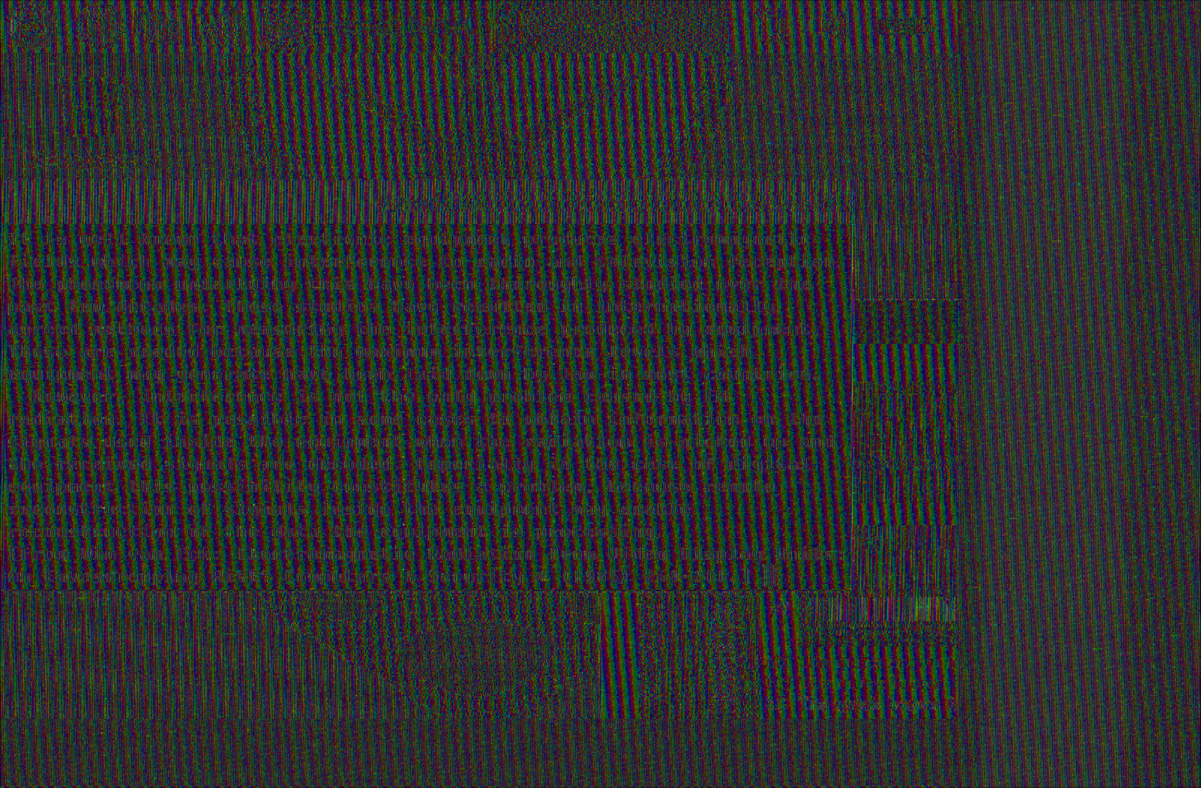
\includegraphics[width=0.7\linewidth]{figures/rawphase.png}
    \caption{HSV representation of reconstruction without unrotation}
    \label{fig:rawphase_hsv}
\end{figure}

Looking at the spectrogram of the raw IQ data in \autoref{fig:rawphase_spectrogram} we see spectral peaks at integer multiples of $f_p$ after the shift by $f_c$, the central frequency of the recording. We can therefore "unrotate" the data by moving one of these peaks to $0$Hz, which will remove the periodic colour bands in the reconstructed image. To do so, we can multiply the raw IQ data by a complex phasor rotating at a frequency of $f_u = f_c - k \cdot f_p$ for some integer $k$, as the spectral peak of the pixel clock is originally at $k \cdot f_p - f_c$. We choose $k$, such that $\mid k \cdot f_p - f_c \mid$ is minimal, i.e., we look at the pixel clock peak closest to the centre frequency.

\begin{figure}[htb]
\centering
\begin{subfigure}{.475\textwidth}
    \centering
    \includesvg[width=\linewidth]{figures/rawphase_spectrogram.svg}
    \caption{Before unrotation}
    \label{fig:rawphase_spectrogram}
\end{subfigure}
\hfill
\begin{subfigure}{.475\textwidth}
    \centering
    \includesvg[width=\linewidth]{figures/unrotated_spectrogram.svg}
    \caption{After unrotation}
    \label{fig:unrotated_spectrogram}
\end{subfigure}

\caption{Spectrograms of roughly the first frames before and after phase unrotation}
\label{fig:rawphase}
\end{figure}

This unrotation decreases colour banding significantly and a single frame contains no visual disruption as seen in \autoref{fig:unrotated_oneframe}. However, across multiple frames, there is still some remaining, as seen in \autoref{fig:unrotated_50frames} which is produced by taking $10$ rows from each of the first $50$ frames. This makes it infeasible to average these frames, as the image quality does not improve significantly (arguably even worsens).

\begin{figure}[htb]
\centering
\begin{subfigure}{.452696\textwidth}
    \centering
    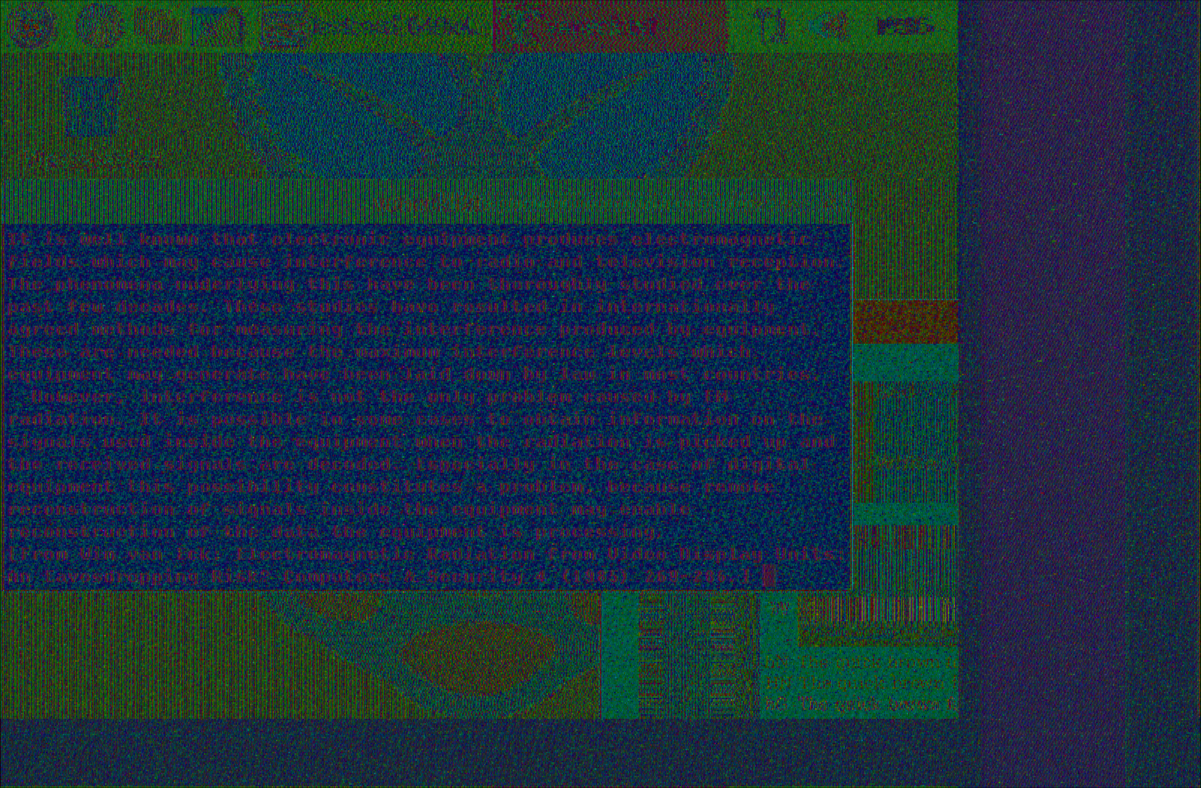
\includegraphics[width=\linewidth]{figures/Unrotated_oneframe.png}
    \caption{One frame}
    \label{fig:unrotated_oneframe}
\end{subfigure}
\hfill
\begin{subfigure}{.475\textwidth}
    \centering
    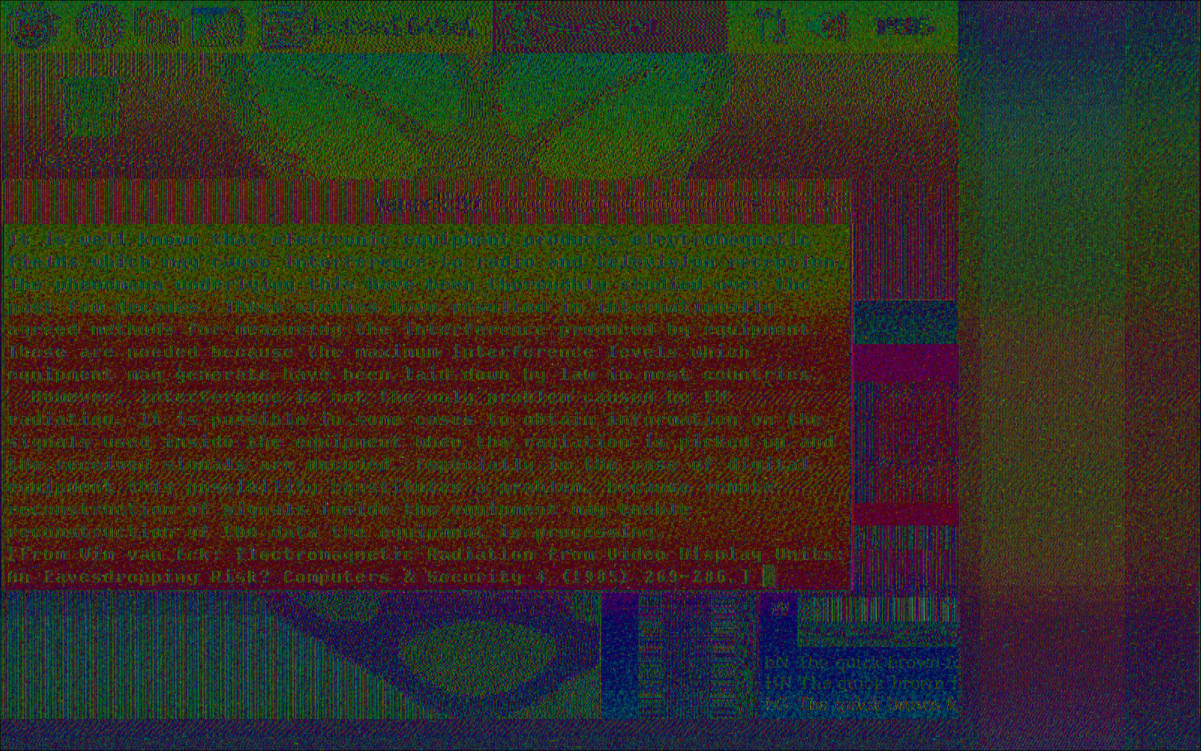
\includegraphics[width=\linewidth]{figures/Unrotated_50frames.png}
    \caption{10 rows from each of the first 50 frames} 
    \label{fig:unrotated_50frames}
\end{subfigure}

\caption{Reconstructions after unrotating by $f_c - k \cdot f_p$}
\label{fig:unrotated}
\end{figure}

This is due to the fact that our unrotation frequency $f_u$ is not accurate enough, probably because of small inaccuracies in $f_p$, which get multiplied by $k$, and become larger inaccuracies. To resolve this issue, we use the following, method to get a better unrotation frequency $f_u^*$. 

First, we want to band-pass the signal, so that only frequencies near $k \cdot f_p - f_c$ remain. As we do not want to keep the frequencies around the frequency $f_c - k \cdot f_p$, we cannot use a regular band-pass filter as that would preserve these as well. Instead, we frequency shift the signal $f_u = f_c - k \cdot f_p$ by multiplying with a complex phasor with this frequency, apply a low-pass filter of a small width (after some experimentation we set the cut-off frequency at $25$Hz) and frequency shift the signal back by $-f_u$. 

After getting this band-passed signal, we perform FM demodulation to measure the actual pixel clock frequency more accurately. Due to noise, there is some local fluctuation in the FM demodulated frequency, which results in a poor visual result after reconstruction. To combat this, we average the FM demodulated values out over each frame and use the frame-specific $f_u^*$ to unrotate the phase of each frame. We also drop the first 2 frames after the unrotation, as the demodulated IQ signal contains some artefacts at the beginning, probably due to the filter properties from the low passing.

This more accurate, per-frame $f_u^*$ unrotation provides an unrotation with virtually no colour banding across the entire recording, which allows us to coherently average all frames in the recording before display

\subsection{Stitching recordings}
\label{sec:stitching}

HDMI transmits $8$-bit colour values of the pixels as $10$-bit words using Transition Minimized Differential Signalling. The result of this is that the actual bit rate over the cable is $10 \times f_p$. As the raster image pixels are sampled with a frequency of $f_p$, the information about it will be reconstructable at any integer multiple of $f_p$. However, due to the fact that bits are transmitted at a frequency of $10 \times fp$, these samples will differ everywhere, whereas every $10 \times f_p$ we will get the exact same emissions, due to the highest sampling rate being $10 \times f_p$ for the bits.

The recording device used to produce the recordings only captures a $40$MHz bandwidth at a time, so to get a better quality reconstruction we can stitch together multiple of these recordings from different centre frequencies, to get one with a larger bandwidth. Namely, we combine the recordings with centre frequencies between $350$MHz and $475$MHz as these seemed to have the best individual reconstructions. We perform the following steps in order to achieve this:

\begin{enumerate}

    \item \textbf{Alignment} \par 
    As all the recordings start at a different point within some frame, we first have to align all of them. We do so by ensuring all of their first samples correspond to the top-left corner of a frame by using the method described in \sectionref{alignment}
    
    \item \textbf{Resampling} \par 
    The original recordings were sampled at $f_s = 64$MHz, however, this sampling frequency can only fit frequencies between $-\frac{f_s}{2}$ and $\frac{f_s}{2}$, i.e. a bandwidth of $64$MHz. If we want to stitch recordings together we require a larger bandwidth, and hence a larger sampling frequency. 

    By stitching together recordings with centre frequencies between $350$MHz and $475$Mhz, we will have some recording content from $330-495$MHz, i.e. a bandwidth of $165$MHz. To fit this, we use a resampled frequency of $192$MHz, and resample as described in \sectionref{resampling}.

    \item \textbf{Filtering} \par 
    As a result of resampling, we get some aliasing, where the frequency profile is repeated 3 times as we had a resampling ratio of 3. To counter this we need to apply a low-pass filter to only keep frequencies with an absolute value of at most $20$MHz.

    However, we also want to apply a low-pass filter to stitch together the frequency domains of different recordings. The centre frequencies are $25$MHz apart, and we do not want two recordings to overlap, as that would increase the strength of the signal in those overlaps by a factor of 2, thus for each recording we only want to keep frequencies between $-12.5$ and $12.5$MHz. As this is a narrower band, we can actually skip the previous low-pass filtering step and only apply this one.

    To ensure that the gain is $0$ at every frequency, we want to use a Linkwitz-Riley filter, as adding up two signals filtered with this kind of filter results in a flat gain profile. This can be realised by cascading two Butterworth filters, which is exactly what Julia's \texttt{filtfilt} function does.

    Note that the bottom-most and top-most centre frequency would only have to be filtered to $20$MHz instead of $12.5$MHz from the bottom and the top respectively, however, for ease of implementation we omit this step, and just filter them to $12.5$MHz as well, as this does not lose too much information, and we are still left with a bandwidth of $165 - 15 = 150$MHz.

    \item \textbf{Frequency shifting} \par 
    Finally, to correctly stitch together the filtered frequency domains, we need to shift each to its actual location in the new frequency domain. As we have centre frequencies between $350$MHz and $475$MHz, the centre frequency of the stitched recording is going to be $\frac{350 + 475}{2} = 412.5$MHz. 

    Therefore for an original recording with centre frequency $f_c$, we multiply it with a complex phasor of frequency $f_c - 412.5$, so that it appears in the correct frequency band in the stitched recording.

    \item \textbf{Summing} \par 
    Finally, we simply add up all the processed recordings, as the Fourier transform is linear, and hence adding up the time-domain samples results in adding up the frequency domains too, and we get the correctly merged frequency domain.
    
\end{enumerate}

\autoref{fig:merged_iq} shows the spectrogram of the stitched-together recording.

\begin{figure}[hbt]
    \centering
    \includesvg[width=.8\linewidth]{figures/merged_iq.svg}
    \caption{Spectrogram of 6 recordings stitched together with a new centre frequency of $412.5$MHz and a sampling rate of $192$MHz.}
    \label{fig:merged_iq}
\end{figure}


\section{Results}
\label{sec:results}

\subsection{Main results}

We have run all of the above algorithms for all the provided recordings with centre frequencies ranging between $225$ and $475$MHz, in addition to the stitched recording created by the methods described in \sectionref{stitching}. As a general trend lower frequencies seemed to yield a worse reconstruction, which probably means a worse signal-to-noise ratio, somewhat confirmed in \sectionref{noise}. \autoref{table:reconstructions} contains some of the more notable reconstructions, either because of their good or poor quality. All of the reconstructed images are available at \url{https://github.com/bazsi700/dsp-assignment4a}.

%%%%% ADD GITHUB BOTH HERE AND IN IMPL

\begin{table}[!htb]
    \centering
    \begin{tblr}{%
        colspec = {Q[c,m,.15\linewidth] Q[c,m,.38\linewidth] Q[c,m,.38\linewidth]},
        width = \linewidth
      }
    \textbf{Frequency} & \textbf{Greyscale} & \textbf{HSV} \\
    
    \hline
    
    Stitched &
    \raisebox{-.5\height}{
    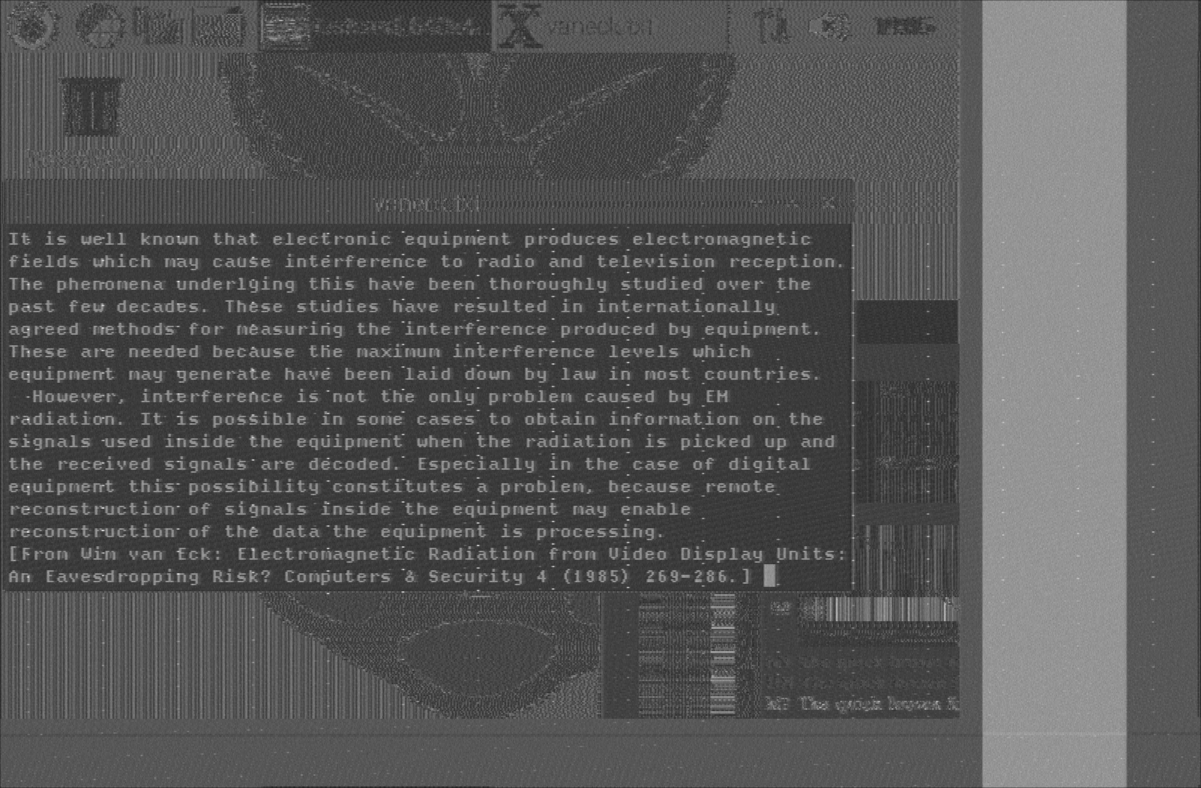
\includegraphics[width=\linewidth]{figures/merged_grayscale.png}
    }
    &
    \raisebox{-.5\height}{
    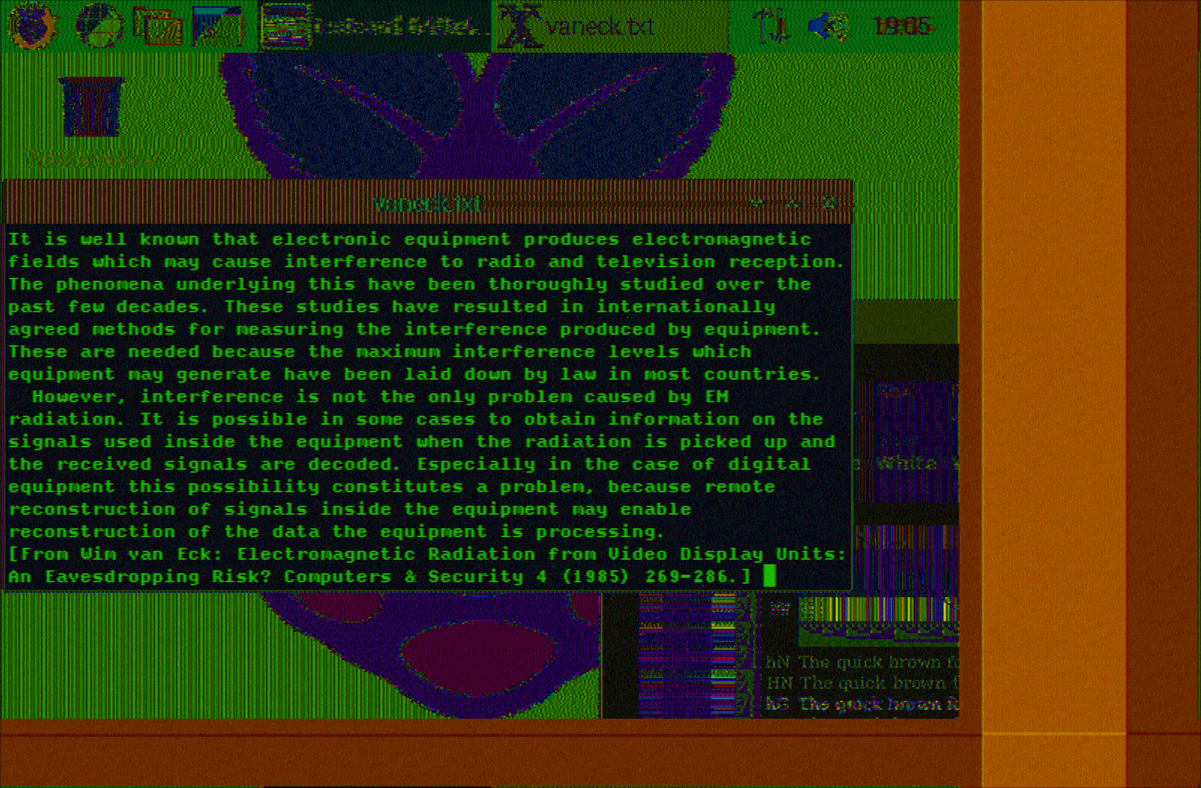
\includegraphics[width=\linewidth]{figures/merged_best_reconstruction.png}
    }
    \\

    
    $475$MHz  &
    \raisebox{-.5\height}{
    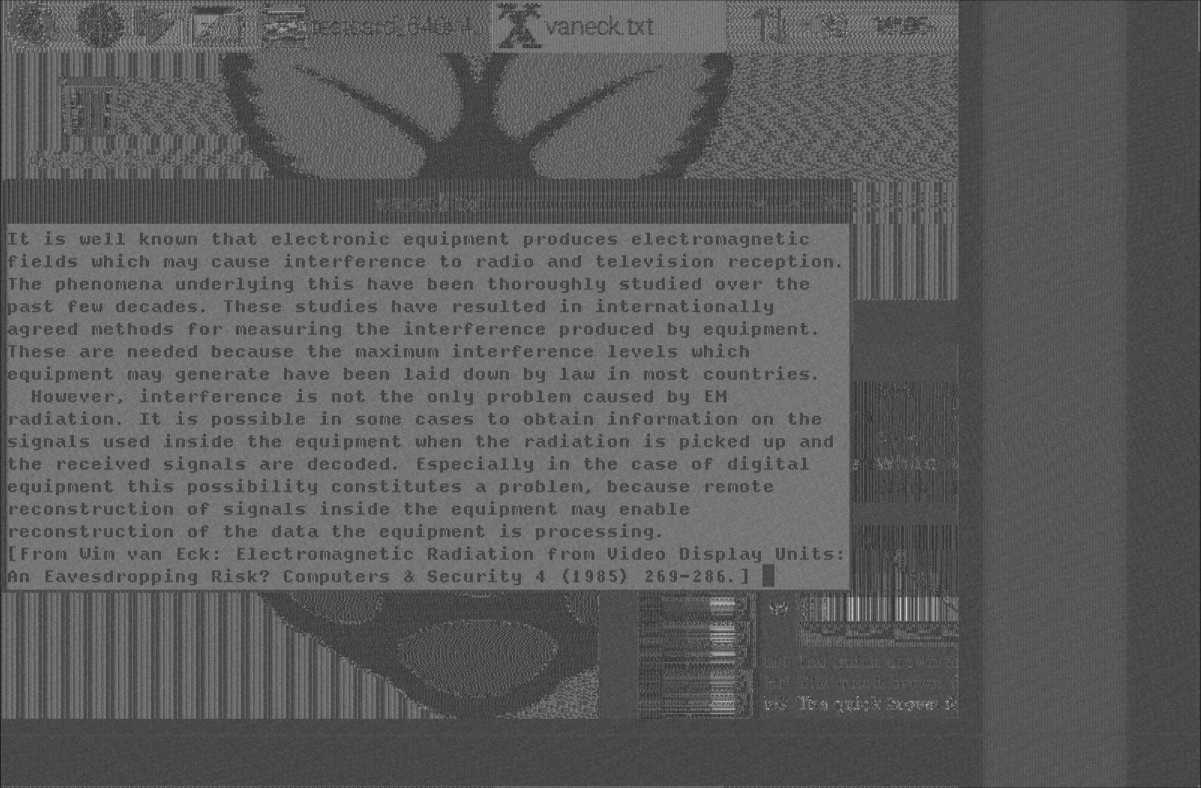
\includegraphics[width=\linewidth]{figures/475_grayscale.png}
    }
    &
    \raisebox{-.5\height}{
    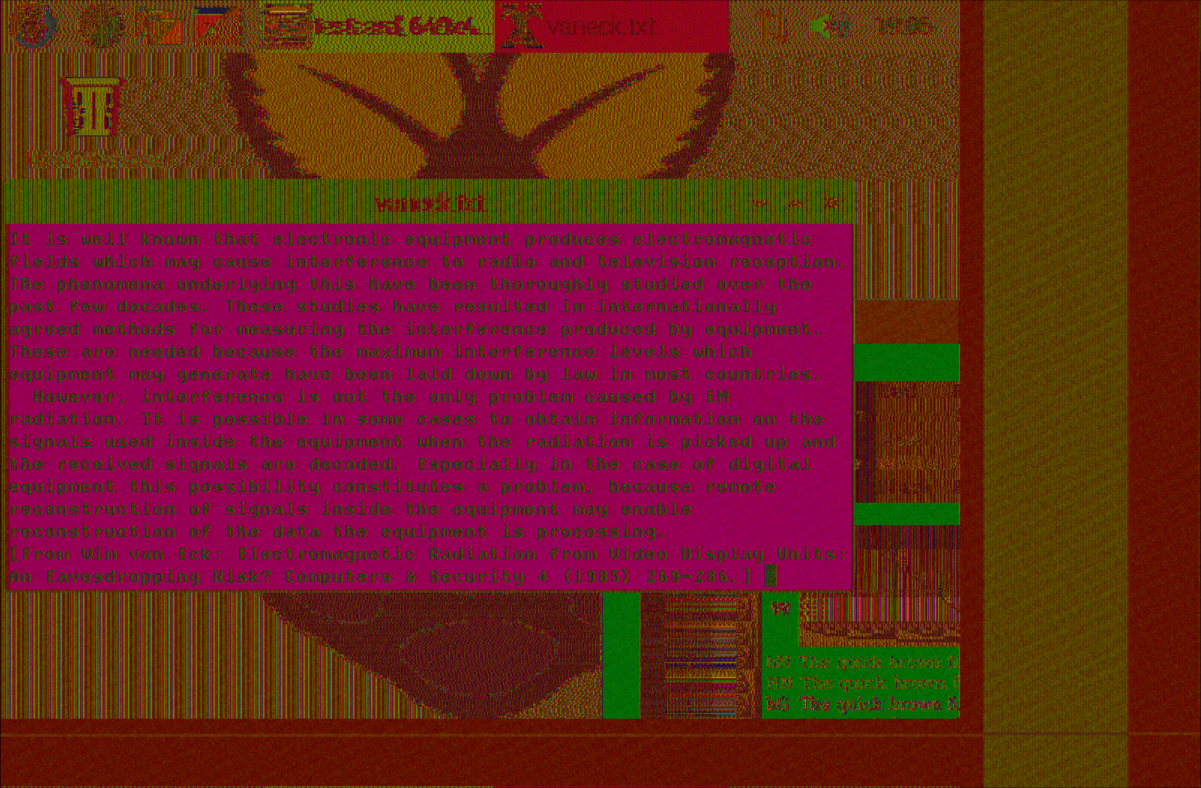
\includegraphics[width=\linewidth]{figures/475_best_reconstruction.png}
    }
    \\

    
      
    $400$MHz  &
    \raisebox{-.5\height}{
    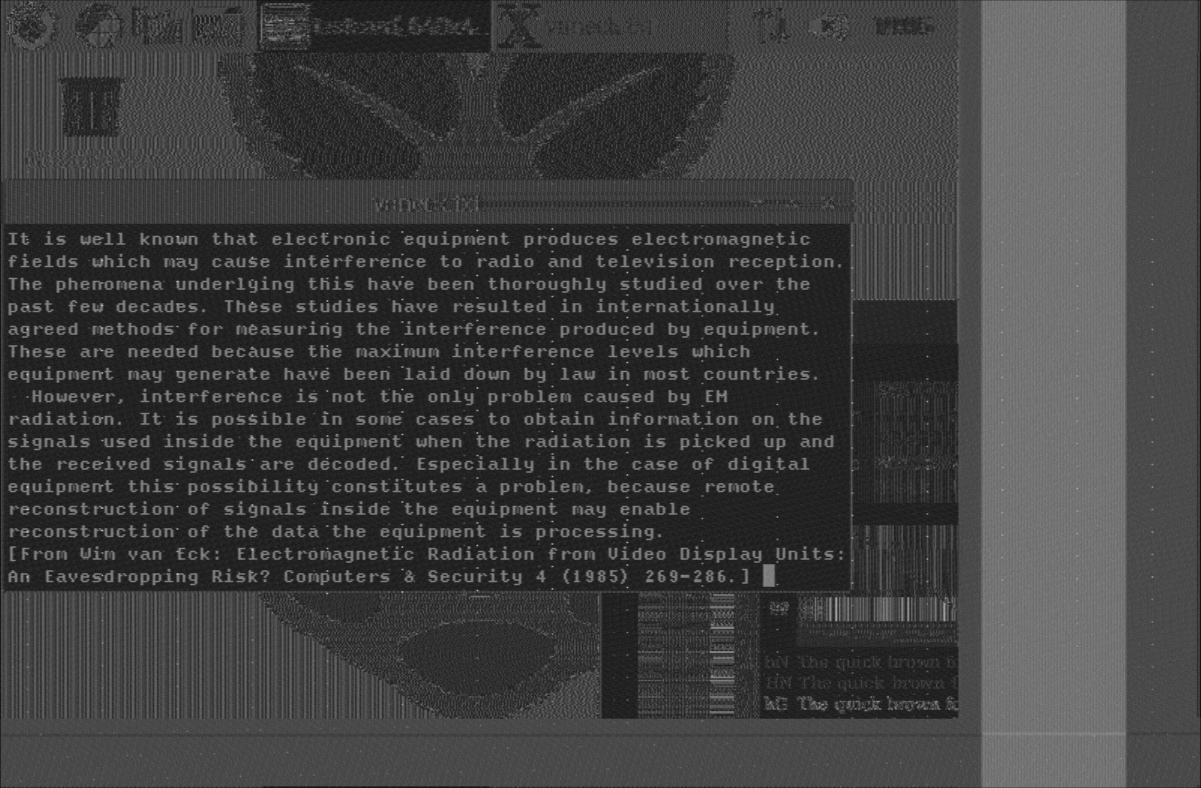
\includegraphics[width=\linewidth]{figures/400_grayscale.png}
    }
    &
    \raisebox{-.5\height}{
    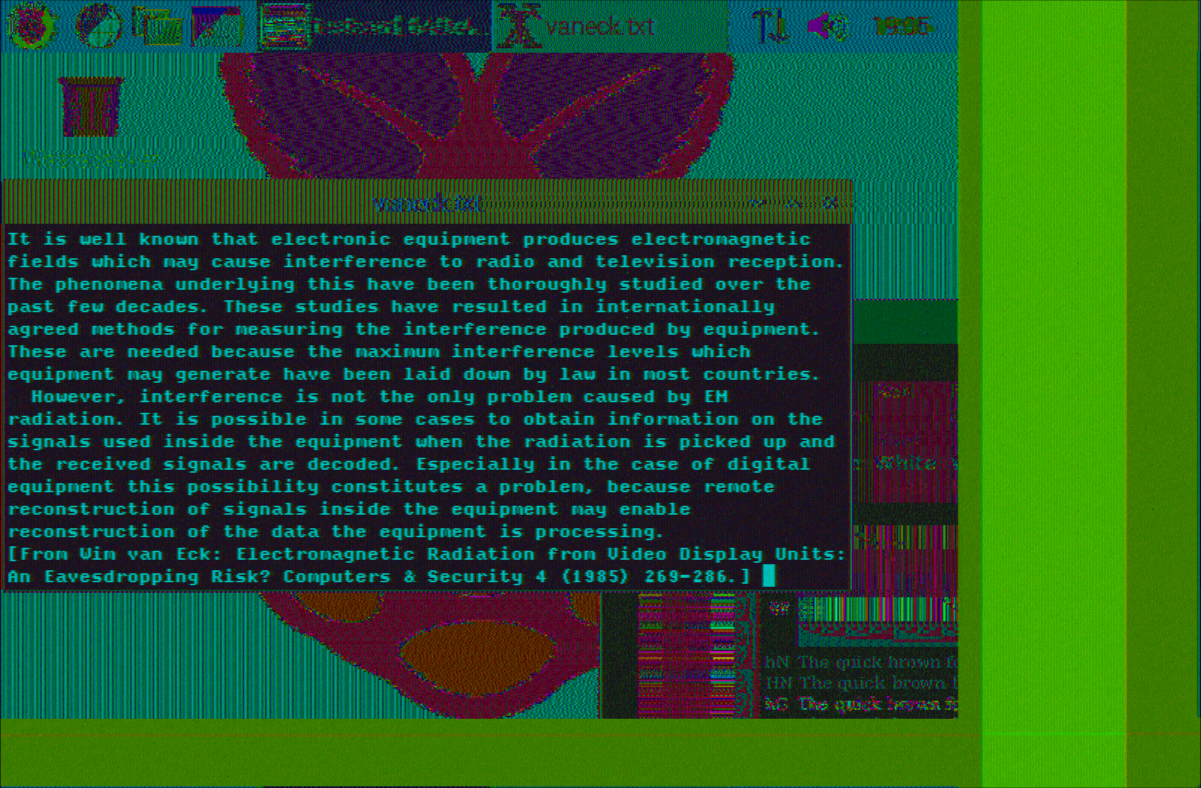
\includegraphics[width=\linewidth]{figures/400_best_reconstruction.png}
    }
    \\

     
    $250$MHz  &
    \raisebox{-.5\height}{
    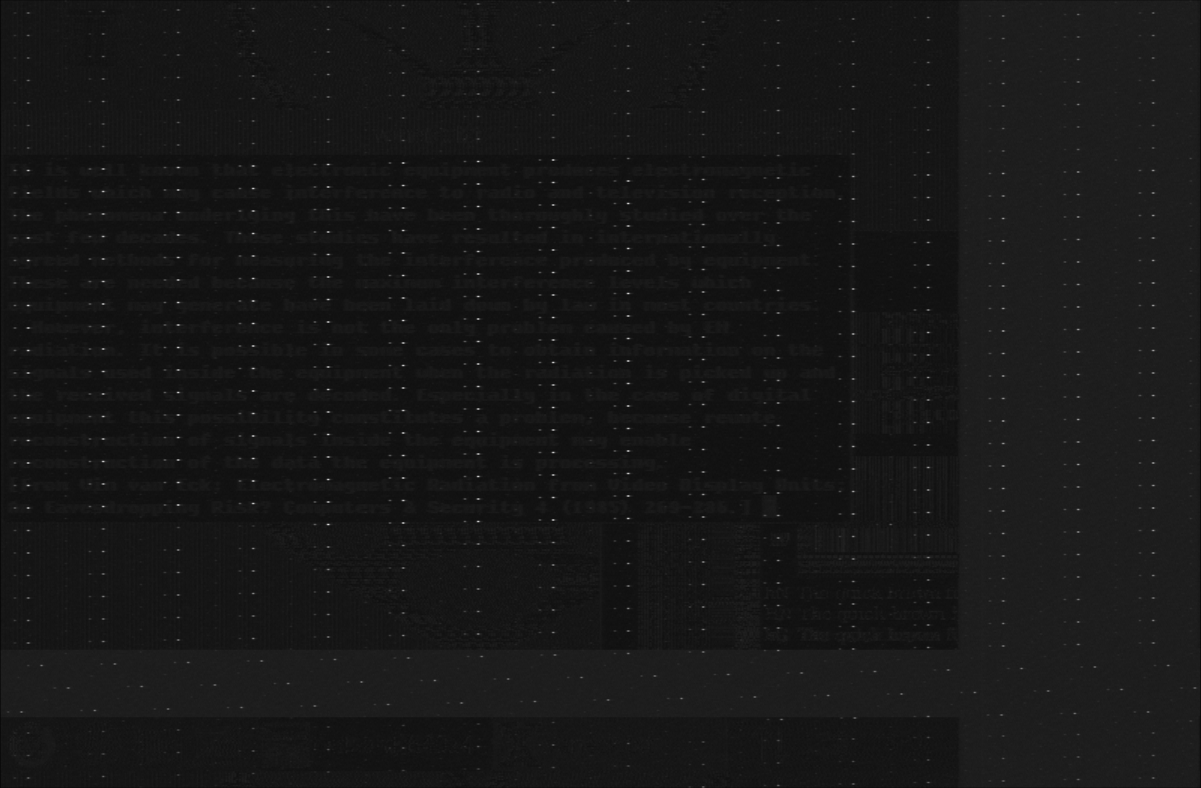
\includegraphics[width=\linewidth]{figures/250_grayscale.png}
    }
    &
    \raisebox{-.5\height}{
    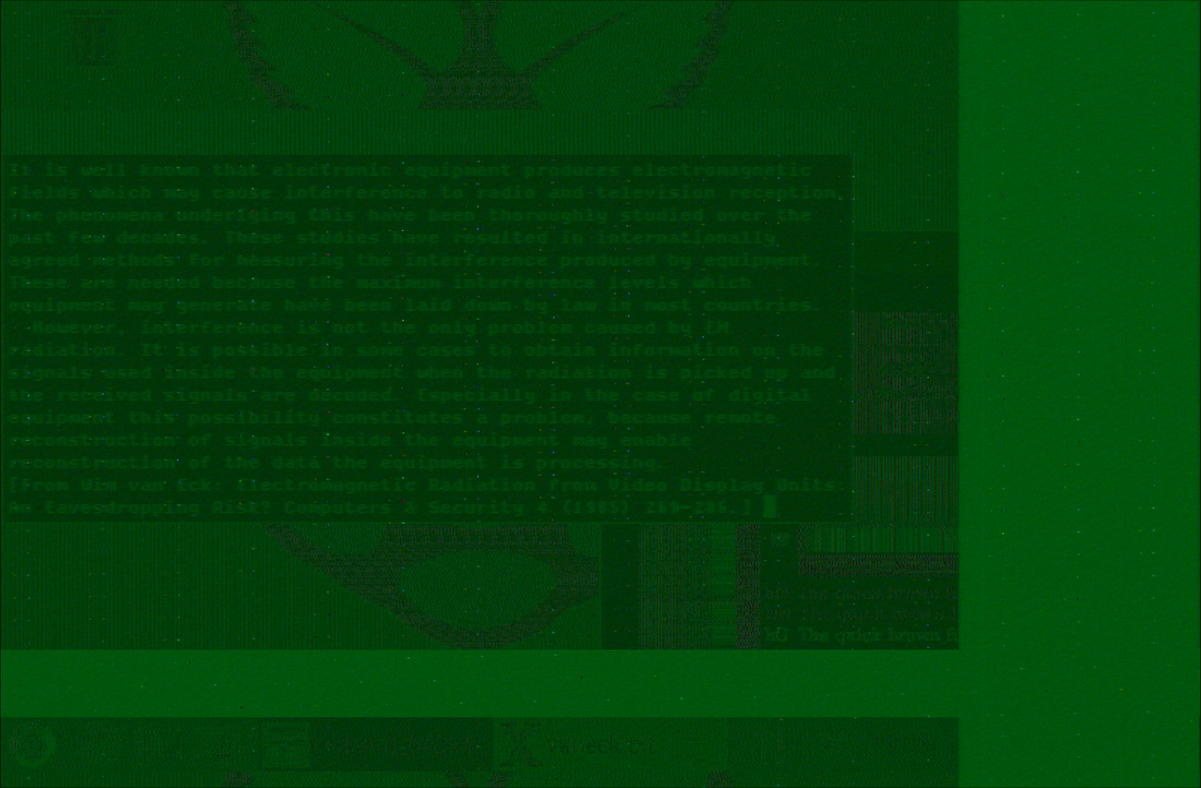
\includegraphics[width=\linewidth]{figures/250_best_reconstruction.png}
    }
    \\
    
    
    $225$MHz  &
    \raisebox{-.5\height}{
    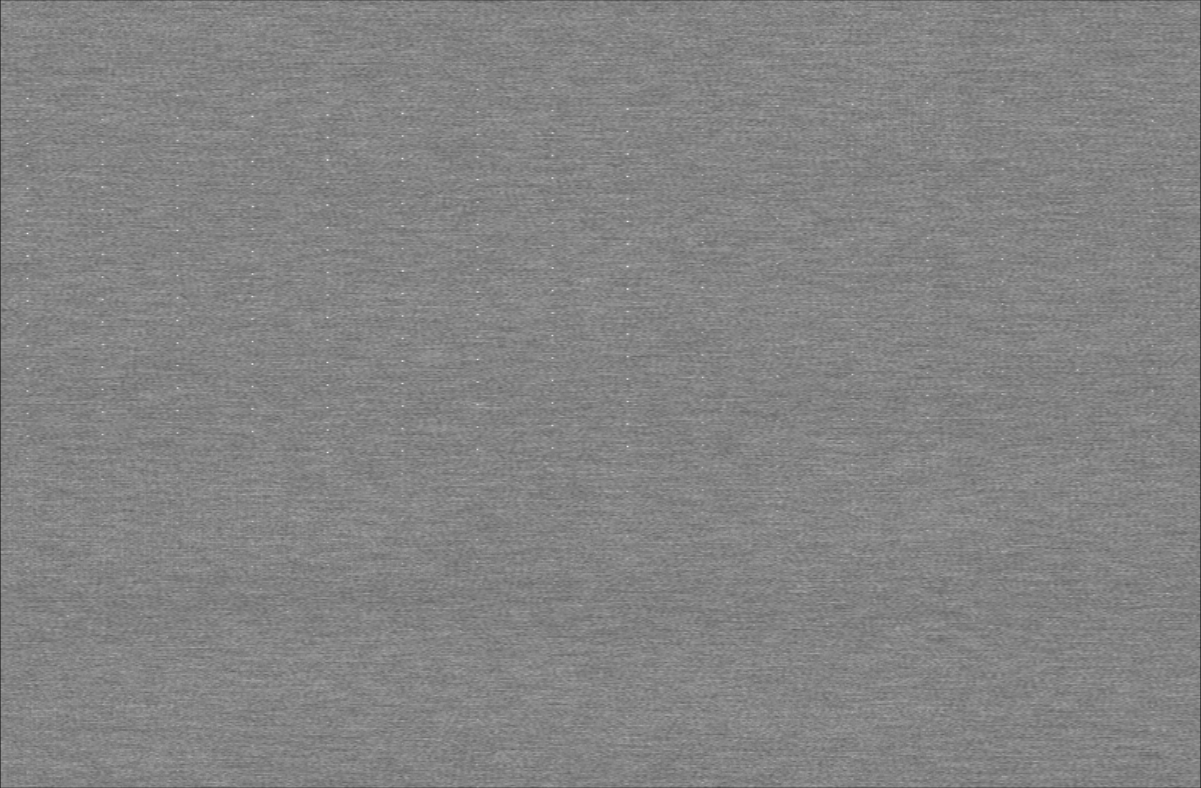
\includegraphics[width=\linewidth]{figures/225_grayscale.png}
    }
    &
    \raisebox{-.5\height}{
    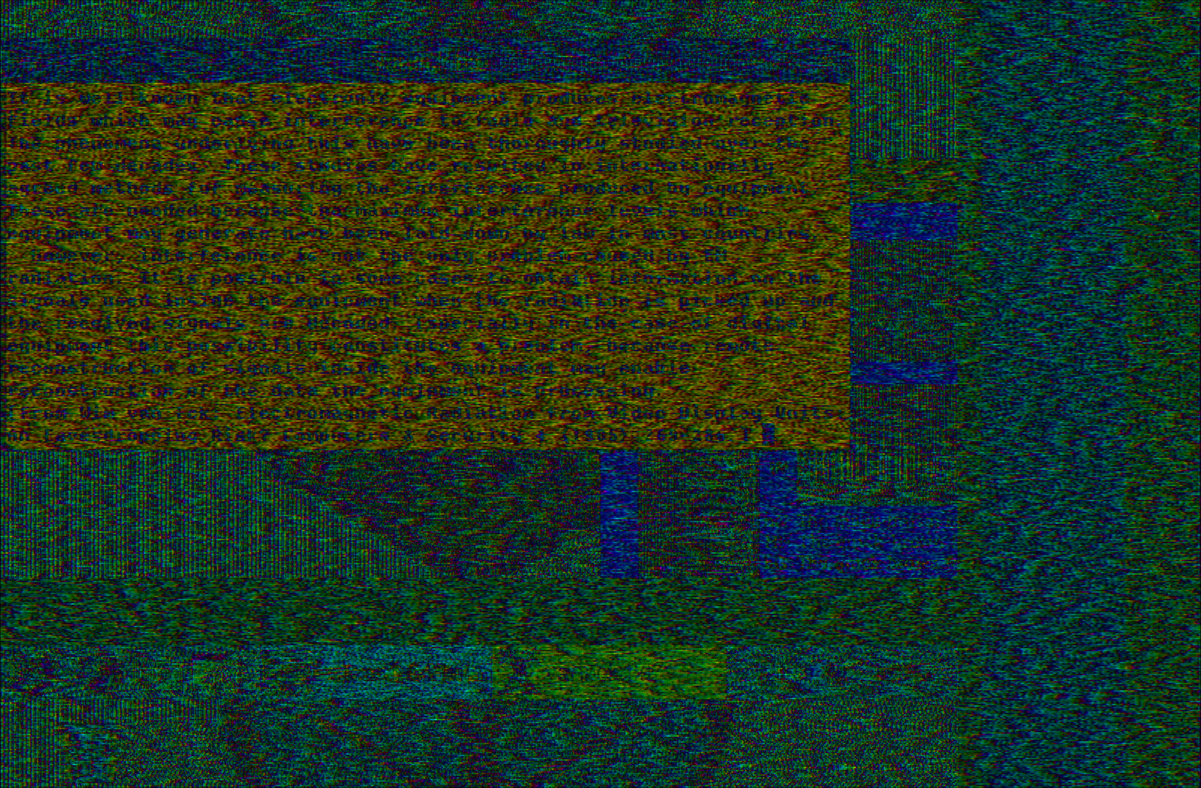
\includegraphics[width=\linewidth]{figures/225_best_reconstruction.png}
    }
    \\


      
    
    \end{tblr}
    \caption{Some of the more notable reconstructions}
    \label{table:reconstructions}
\end{table}

\subsection{Noise}
\label{sec:noise}

\subsubsection{Background noise}

Besides the recordings containing the electromagnetic radiation from the HDMI cable, we were also provided with recordings of the background noise with the target device turned off. To measure the level of background noise, we compared the signal intensity of the two recordings from the same centre frequency, the one with the target device switched on and the one with it off. We used the root-mean-square (RMS) signal strength to measure the signal intensity in all of the recordings. \autoref{fig:scene_to_noise} shows the ratio between the scene (target device on) recording's RMS and the noise recording's RMS for each of the centre frequencies.

\begin{figure}[hbt]
    \centering
    \includesvg[width=.7\linewidth]{figures/scene_to_noise.svg}
    \caption{Ratio of scene and noise RMS-es.}
    \label{fig:scene_to_noise}
\end{figure}

We see a pretty low ratio for the centre frequency for $225$MHz, which is consistent with the poor visual results we see in \autoref{table:reconstructions}. Arguably the best reconstruction was at $400$MHz which is the highest scene to noise RMS ratio in the recording as well. We see a large dip at $450$MHz, despite the image reconstruction being decent at this frequency. Plotting the noise RMS-ses are roughly constant between the centre frequencies $250$ and $475$MHz and the main difference is in the scene RMSes, however, there is a spike in noise intensity at $450$MHz. Because of the fact that this does not seem to impact the image reconstruction, our best guess is that there was some additional noise for some external reason at the time the noise recording for $450$MHz was made, which was not present at the scene recording.


\subsubsection{Adding extra noise}

The resilience of our processing methods to noise is somewhat shown by how we lose image quality significantly at lower centre frequencies with more noise. However, to do some more testing we decided to test how the image reconstruction changes when adding more noise to the recording at centre frequency $400$MHz, the one with the least noise originally according to signal intensity ratios.

The way we did this, is took the original scene IQ samples $\{z_n\}$, and the IQ samples from the noise recording $\{\epsilon_n\}$ and produced the sequence $\{z_n^*\} = \{z_n\} + c \cdot \{\epsilon_n\}$ for various noise multipliers of $c$. The results of this can be seen in \autoref{table:noisy_reconstructions}. For $c=4$ the $f_p$ reconstruction described in \sectionref{shearing} fails using non-coherent auto-correlation and thus we switch to a coherent one. For $c \geq 16$ even this fails, and we fall back to manually setting the value of $f_p = 2.520009689e7$ which we get from the $c = 0$ reconstruction.


\begin{table}[htb]
    \centering
    \begin{tblr}{%
        colspec = {Q[c,m,.2\linewidth] Q[c,m,.5\linewidth]},
        width = \linewidth
      }
    \textbf{Noise multiplier ($c$)} & \textbf{HSV} \\
    
    \hline

    $1$ &
    \raisebox{-.5\height}{
    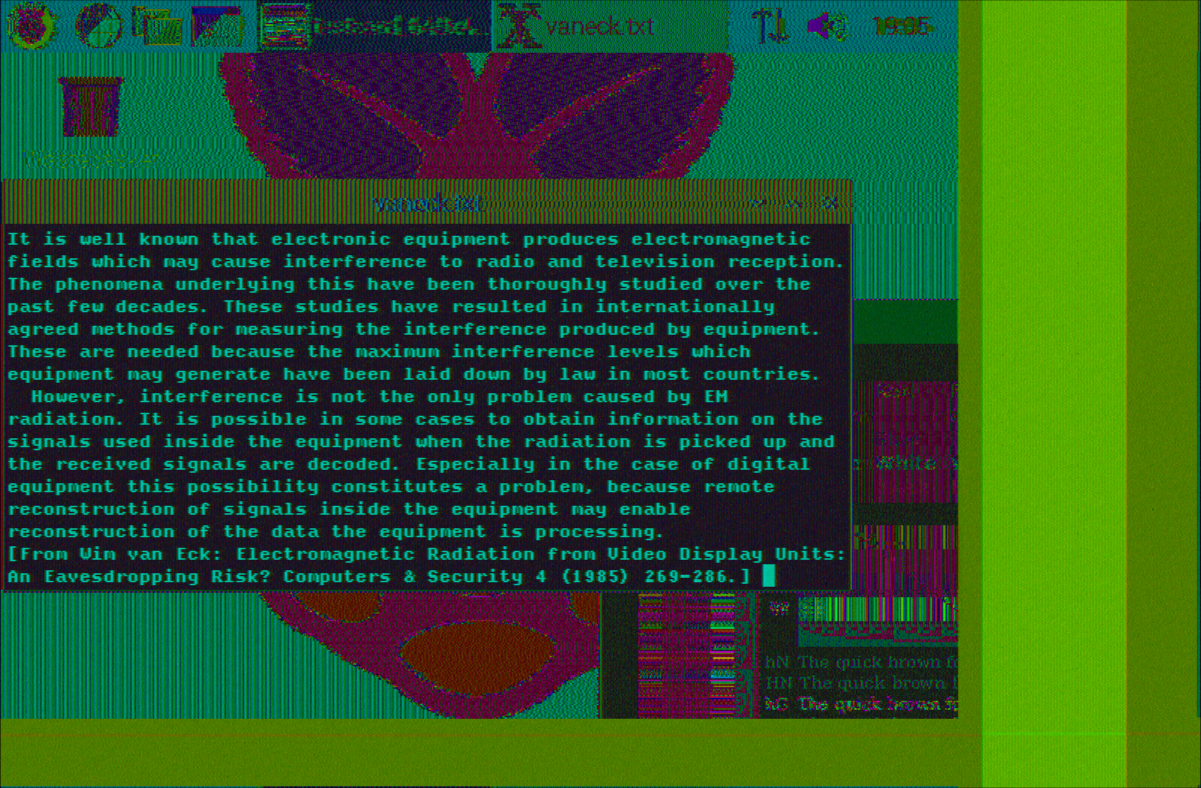
\includegraphics[width=.8\linewidth]{figures/400_1x_noise.png}
    }
    \\

    $4$ &
    \raisebox{-.5\height}{
    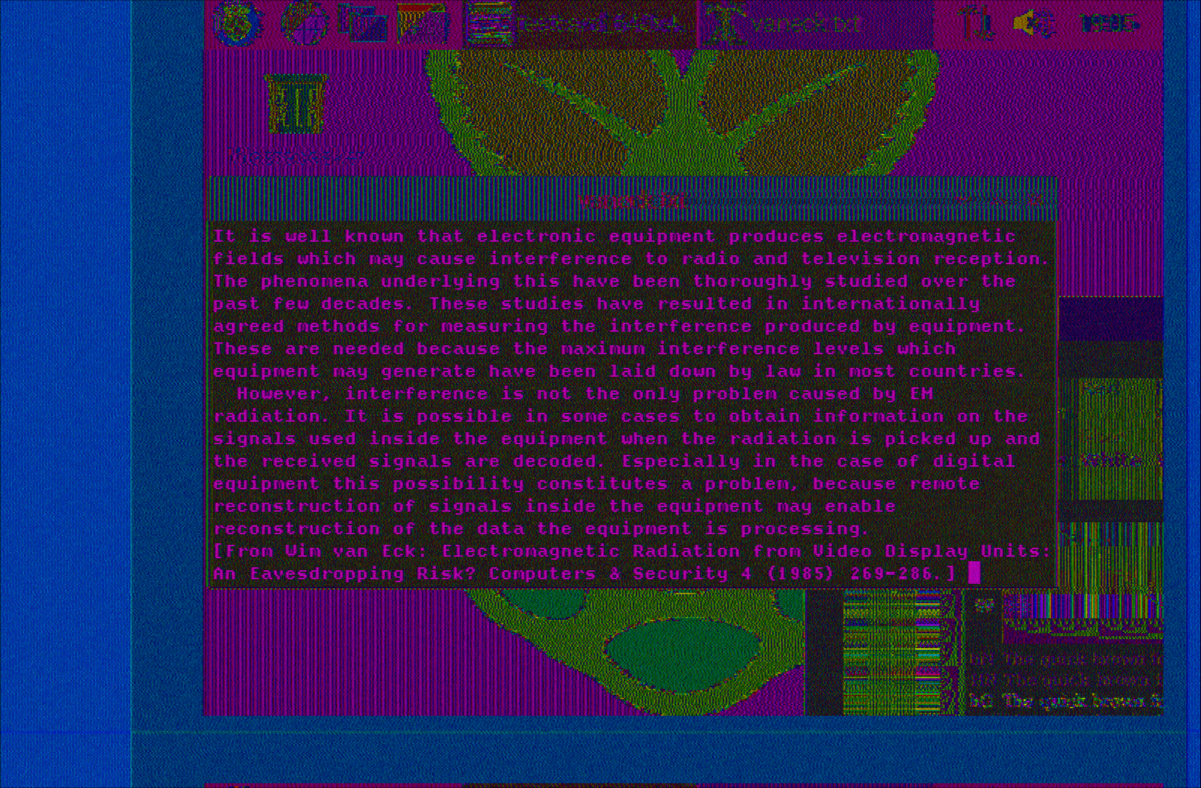
\includegraphics[width=.8\linewidth]{figures/400_4x_noise.png}
    }
    \\

    $16$ &
    \raisebox{-.5\height}{
    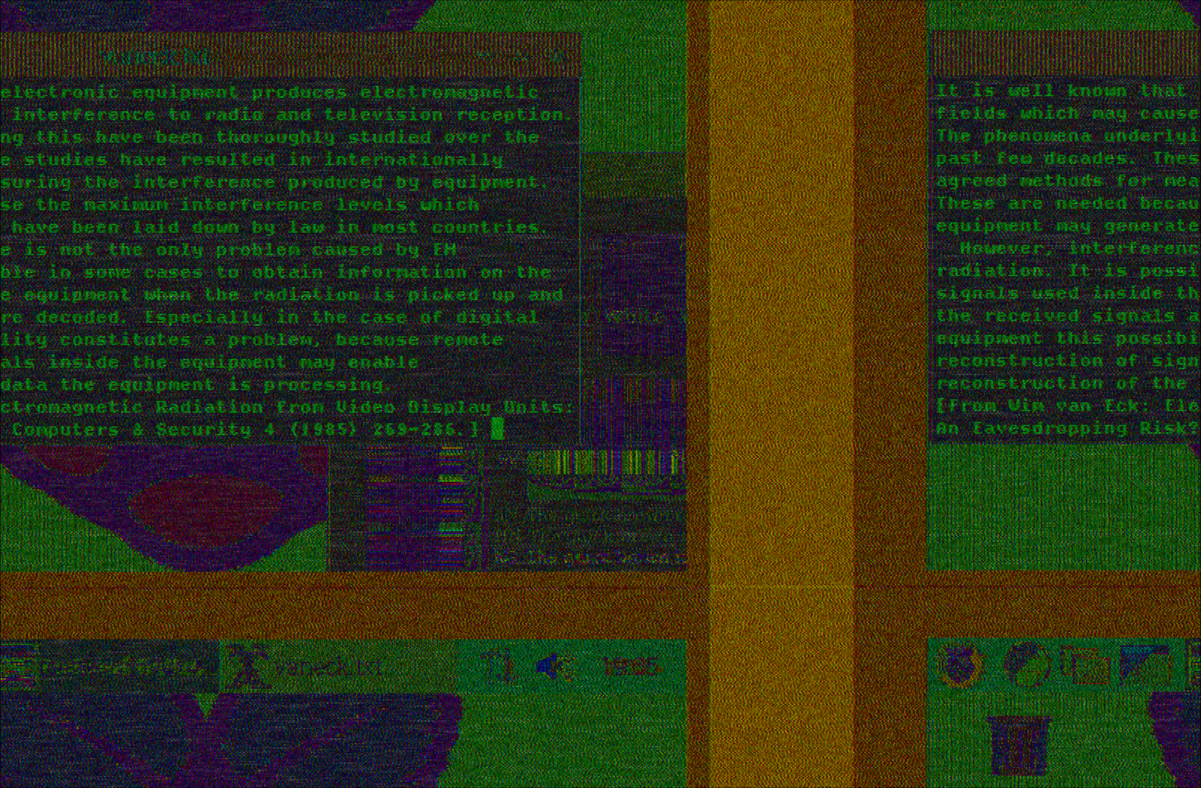
\includegraphics[width=.8\linewidth]{figures/400_16x_noise.png}
    }
    \\
	
	
    $64$ &
    \raisebox{-.5\height}{
    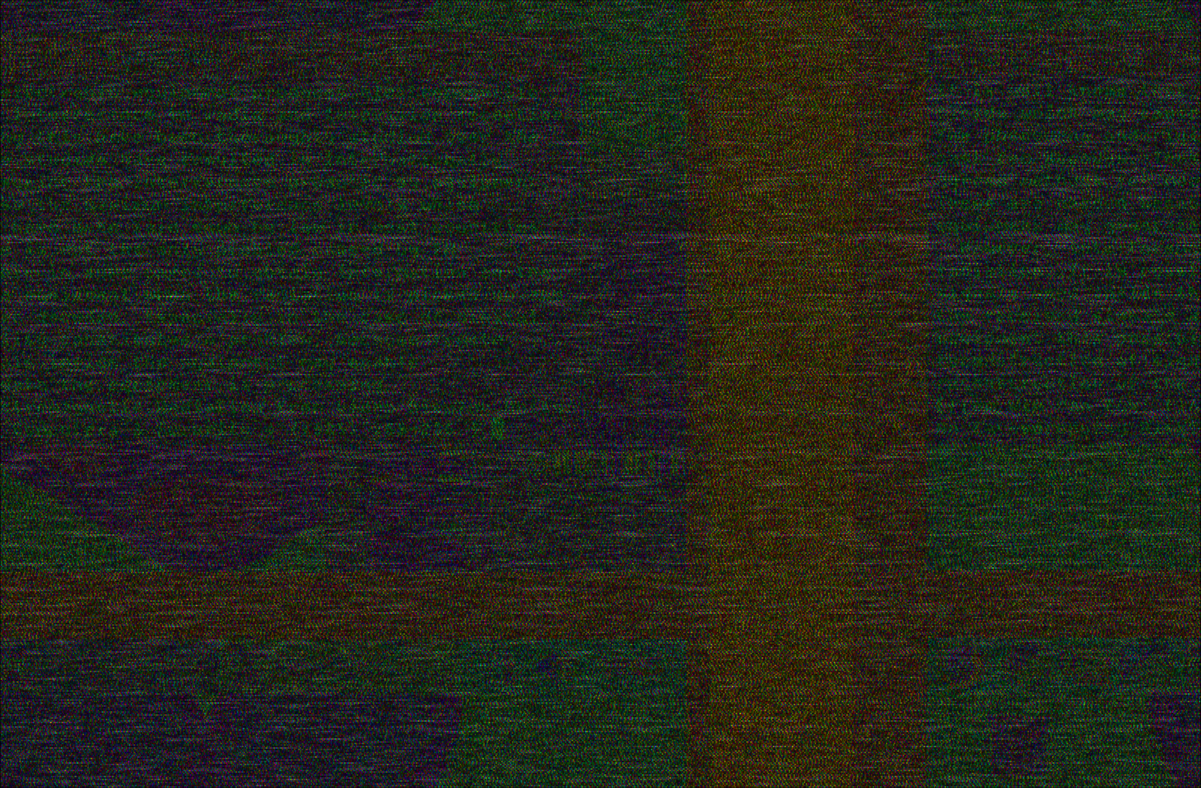
\includegraphics[width=.8\linewidth]{figures/400_64x_noise.png}
    }
    \\
      
      
    
    \end{tblr}
    \caption{Reconstructions at $f_c = 400$MHz with varying levels of added noise}
    \label{table:noisy_reconstructions}
\end{table}


We can see that for $c=1$ we get a very good image quality as the signal-to-noise ratio is still quite high, for $c=4$ the image starts to get grainy and the alignment fails but the overall image quality is still decent, for $c=16$ the image gets grainier, but most of the text is still readable, and for $c=64$ the image is so grainy that only rough outlines of shapes can be seen, but all text is illegible.

\subsection{Different sampling methods}

As described in \sectionref{resampling}, besides linear interpolation, we also tried nearest neighbour resampling and windowed sinc interpolation. The results of nearest neighbour sampling very closely resembled the results of linear interpolation, while windowed sinc interpolation resulted in a blurrier image. Our best guess as to why this is, is that we could only perform sinc interpolation with a relatively small window size (around $20$) in reasonable runtimes, and the weight of the remaining samples not included in the sinc window would have been non-negligible. The image results of reconstruction can be found at \url{https://github.com/bazsi700/dsp-assignment4a}.


\section{Conclusion}
\label{sec:conclusion}

We conclude, that given a $1$ second long recording from a centre frequency without too much noise, the original image transmitted via an HDMI cable can be reconstructed to a level where most text is legible. This can cause a security vulnerability in systems where the transmitted information is sensitive and adversaries have the chance to snoop in the vicinity of the video cable. 

To combat this protective measures should be taken when operating in such an environment, either by coating the cable to shield its emissions or by encrypting the data passing through the cable. Intel has developed a system to do the latter, called High-bandwidth Digital Content Protection (HDCP) whose main purpose is to prevent copying of digital audio and video content when it travels through cables, however, by extension it also prevents snooping.

\end{document}
